%%%%%%%%%%%%%%%%%%%%%%%%%%%%%%%%%%%%%%%%%%%%%%%%%%%%%%%%%%%%%%%%%
%%%%%%%%%%%%%%%%%%%%%%%%%%%%%%%%%%%%%%%%%%%%%%%%%%%%%%%%%%%%%%%%%
\setcounter{chapter}{4}
\newcommand{\graphicscompanion}{\glqq The \LaTeX{} Graphics Companion\grqq~\cite{graphicscompanion}}
\newcommand{\hobby}{\glqq A User's Manual for \MP\grqq~\cite{metapost}}
\newcommand{\hoenig}{\glqq \TeX{} Unbound\grqq~\cite{unbound}}
\newcommand{\graphicsinlatex}{\glqq Graphics in \LaTeXe\grqq~\cite{ursoswald}}

\chapter{Matemaatilise graafika genereerimine}
\label{chap:graphics}\index{joonised}

\begin{intro}
Enamasti kasutatakse \LaTeX i teksti vormistamiseks. Kuid et struktuurne
lähenemine sisuloomele on väga praktiline, sisaldab \LaTeX{} ka
vahendeid, kuigi mõneti piiratuid, tekstkirjelduste järgi graafilise
väljundi genereerimiseks. Lisaks on \LaTeX i jaoks koostatud päris
mitmeid laiendusi, mis püüavad sellest piiratusest üle saada. Käesolevas
peatükis tutvustamegi neist mõningaid.
\end{intro}

\section{Ülevaade}

Graafilise väljundi loomisel \LaTeX iga on pikk traditsioon. See algas
keskkonnaga \ei{picture}, mis võimaldab koostada graafikat
eeldefineeritud elementide paneelile paigutamise teel. Täieliku
kirjelduse annab raamat \manual. \LaTeXe{} keskkond \ei{picture}
sisaldab käsku \ci{qbezier}, kus \texttt{q} tähistab ruutkõverat
(\emph{quadratic}). Paljusid sagedasti kasutatavaid jooni, nagu
ringjooni, ellipseid ja aheljooni saab rahuldavalt lähendada B\'ezier'
ruutkõveratega, kuigi see võib nõuda veidi matemaatilist vaevanägemist.
Kui aga seejuures genereerida \LaTeX i sisendfailide \ci{qbezier}-plokid
programmi abil, muutub keskkond \ei{picture} päris võimsaks.

Olgugi et jooniste programmeerimine otse \LaTeX is on väga piiratud ja
tihti tüütu, leidub siiski põhjusi, miks seda teha. Sedasi moodustatud
dokumendid on baidisuuruse poolest "`väikesed"' ja puuduvad
graafikafailid, mida on vaja kogu aeg kaasas kanda.

Niisugune oli asjade seis kuni hetkeni, mil mõni aasta tagasi valmis
klassi \pai{beamer} autori \index{Tantau, Till}Till Tantau käe all
Portable Graphics Format (pakett \pai{pgf}) ja seonduv kasutajaliides
TikZ (pakett \pai{tikz}). See süsteem võimaldab luua kõrge kvaliteediga
vektorgraafikat kõigis \TeX i süsteemides täieliku PDFi toega.

Sellele baasile tuginedes on kirjutatud palju pakette mitmesugusteks
otstarveteks. Laia valikut nendest pakettidest tutvustab üksikasjaliselt
\graphicscompanion{}.

Ilmselt kõige arenenum \LaTeX iga seotud graafikatööriist on
\index{metapost@\MP}\MP. See on eraldiseisev rakendus, mis on
\index{Knuth, Donald E.}Donald E. Knuthi kirjutatud programmi
\index{metafont@\MF}\MF\ kaksikõde. \MP i aluseks on \MF i väga võimas
ja matemaatiliselt väljendusrikas programmeerimiskeel, kuid erinevalt
programmist \MF{} genereerib ta kapseldatud \PSi i faile, mida saab
lisada \LaTeX i ja isegi pdf\LaTeX i. Sissejuhatuse leiab manuaalist
\hobby{} või juhendist \cite{ursoswald}.

Väga põhjaliku käsitluse \LaTeX i ja \TeX i graafika- (ja kirja-)
strateegiatest leiab raamatust \hoenig.

\section{Keskkond \ei{picture}}
\secby{Urs Oswald}{osurs@bluewin.ch}
Nagu ülal mainitud, on keskkond \ei{picture} osa standard-\LaTeX ist
ja sobib väga hästi lihtsate ülesannete jaoks ning juhuks, kui on vaja
leheküljel täpset kontrolli üksikute elementide üle. Tõsisema
graafikatöö puhul tuleks aga vaadata paketi TikZ poole, mida
tutvustatakse jaotises \ref{sec:tikz} leheküljel \pageref{sec:tikz}.

\subsection{Põhikäsud}

Keskkond \ei{picture}\footnote{Usu või ära usu, aga keskkond
\ei{picture} töötab standard-\LaTeX is niisama, ilma et oleks vaja
sisse lugeda ühtki paketti.} luuakse ühega järgmisest kahest käsust:
\begin{lscommand}
\verb|\begin{picture}(|$x,y$\verb|)| \ldots\verb|\end{picture}|
\end{lscommand}
\noindent või
\begin{lscommand}
\verb|\begin{picture}(|$x,y$\verb|)(|$x_0,y_0$\verb|)| \ldots\verb|\end{picture}|
\end{lscommand}
\noindent Arvud $x$, $y$, $x_0$, $y_0$ viitavad ühikpikkusele
\ci{unitlength}, millele saab igal hetkel (kuid mitte keskkonna
\ei{picture} sees) anda väärtustamiskäsuga uue väärtuse, nagu näiteks
\begin{lscommand}
\ci{setlength}\verb|{|\ci{unitlength}\verb|}{1.2cm}|
\end{lscommand}
\noindent Ühikpikkuse \ci{unitlength} vaikeväärtus on \texttt{1pt}.
Esimene paar $(x,y)$ reserveerib dokumendis joonise jaoks
ristkülikukujulise ruumi. Valikuline teine paar $(x_0,y_0)$ omistab
reserveeritud ristküliku alumisele vasakule nurgale suvalised
koordinaadid.

Enamik joonistamiskäske on ühel kahest kujust:
\begin{lscommand}
\ci{put}\verb|(|$x,y$\verb|){|\emph{objekt}\verb|}|
\end{lscommand}
\noindent või
\begin{lscommand}
\ci{multiput}\verb|(|$x,y$\verb|)(|$\Delta x,\Delta y$\verb|){|$n$\verb|}{|\emph{objekt}\verb|}|\end{lscommand}
\noindent Erandiks on B\'ezier' kõverad, mida joonistatakse käsuga
\begin{lscommand}
\ci{qbezier}\verb|(|$x_1,y_1$\verb|)(|$x_2,y_2$\verb|)(|$x_3,y_3$\verb|)|
\end{lscommand}

\subsection{Lõigud}

\begin{example}
\setlength{\unitlength}{5cm}
\begin{picture}(1,1)
  \put(0,0){\line(0,1){1}}
  \put(0,0){\line(1,0){1}}
  \put(0,0){\line(1,1){1}}
  \put(0,0){\line(1,2){.5}}
  \put(0,0){\line(1,3){.3333}}
  \put(0,0){\line(1,4){.25}}
  \put(0,0){\line(1,5){.2}}
  \put(0,0){\line(1,6){.1667}}
  \put(0,0){\line(2,1){1}}
  \put(0,0){\line(2,3){.6667}}
  \put(0,0){\line(2,5){.4}}
  \put(0,0){\line(3,1){1}}
  \put(0,0){\line(3,2){1}}
  \put(0,0){\line(3,4){.75}}
  \put(0,0){\line(3,5){.6}}
  \put(0,0){\line(4,1){1}}
  \put(0,0){\line(4,3){1}}
  \put(0,0){\line(4,5){.8}}
  \put(0,0){\line(5,1){1}}
  \put(0,0){\line(5,2){1}}
  \put(0,0){\line(5,3){1}}
  \put(0,0){\line(5,4){1}}
  \put(0,0){\line(5,6){.8333}}
  \put(0,0){\line(6,1){1}}
  \put(0,0){\line(6,5){1}}
\end{picture}
\end{example}

Lõike joonistatakse käsuga
\begin{lscommand}
\ci{put}\verb|(|$x,y$\verb|){|\ci{line}\verb|(|$x_1,y_1$\verb|){|$pikkus$\verb|}}|
\end{lscommand}
\noindent Käsul \ci{line} on kaks argumenti: suunavektor ja pikkus.
Suunavektori komponendid piirduvad täisarvudega
\[
  -6,\,-5,\,\ldots,\,5,\,6,
\]
ja nad peavad olema ühistegurita (pole muid ühiseid tegureid peale 1).
Joonisel on kujutatud kõik 25 võimalikku kalde väärtust esimeses
veerandis. Pikkus määratakse ühikpikkuse \ci{unitlength} suhtes. Pikkuse
argument on vertikaaljoone puhul vertikaalkoordinaat ja kõigil ülejäänud
juhtudel horisontaalkoordinaat.

\subsection{Nooled}

\begin{example}
\setlength{\unitlength}{0.75mm}
\begin{picture}(60,40)
  \put(30,20){\vector(1,0){30}}
  \put(30,20){\vector(4,1){20}}
  \put(30,20){\vector(3,1){25}}
  \put(30,20){\vector(2,1){30}}
  \put(30,20){\vector(1,2){10}}
  \thicklines
  \put(30,20){\vector(-4,1){30}}
  \put(30,20){\vector(-1,4){5}}
  \thinlines
  \put(30,20){\vector(-1,-1){5}}
  \put(30,20){\vector(-1,-4){5}}
\end{picture}
\end{example}
Nooli joonistatakse käsuga
\begin{lscommand}
\ci{put}\verb|(|$x,y$\verb|){|\ci{vector}\verb|(|$x_1,y_1$\verb|){|$pikkus$\verb|}}|
\end{lscommand}
\noindent Noolte puhul on suunavektori komponendid veelgi kitsamalt
piiratud kui lõikude puhul, nimelt täisarvudega
\[
  -4,\,-3,\,\ldots,\,3,\,4.
\]
Komponendid peavad samuti olema ühistegurita (pole muid ühiseid
tegureid peale 1). Võib tähele panna käsu \ci{thicklines}\cih{thinlines}
mõju kahele noolele, mis osutavad üles vasakule.

\subsection{Ringjooned}

\begin{example}
\setlength{\unitlength}{1mm}
\begin{picture}(60, 40)
  \put(20,30){\circle{1}}
  \put(20,30){\circle{2}}
  \put(20,30){\circle{4}}
  \put(20,30){\circle{8}}
  \put(20,30){\circle{16}}
  \put(20,30){\circle{32}}

  \put(40,30){\circle{1}}
  \put(40,30){\circle{2}}
  \put(40,30){\circle{3}}
  \put(40,30){\circle{4}}
  \put(40,30){\circle{5}}
  \put(40,30){\circle{6}}
  \put(40,30){\circle{7}}
  \put(40,30){\circle{8}}
  \put(40,30){\circle{9}}
  \put(40,30){\circle{10}}
  \put(40,30){\circle{11}}
  \put(40,30){\circle{12}}
  \put(40,30){\circle{13}}
  \put(40,30){\circle{14}}

  \put(15,10){\circle*{1}}
  \put(20,10){\circle*{2}}
  \put(25,10){\circle*{3}}
  \put(30,10){\circle*{4}}
  \put(35,10){\circle*{5}}
\end{picture}
\end{example}
Käsk
\begin{lscommand}
  \ci{put}\verb|(|$x,y$\verb|){|\ci{circle}\verb|{|\emph{diameeter}\verb|}}|
\end{lscommand}
\noindent joonistab ringjoone keskpunktiga $(x,y)$ ja diameetriga (mitte
raadiusega) \emph{diameeter}. Keskkond \ei{picture} tunnistab ainult
diameetreid kuni umbes 14\,mm-ni ja ka sellest piirist allpool pole kõik
diameetrid võimalikud. Käsk \ci{circle*} joonistab ketta (täidetud
ringi).

Nagu lõikude puhulgi, võib olla tarvis abiks võtta lisapaketid nagu
\pai{eepic} või \pai{pstricks}. Neid pakette on põhjalikult kirjeldatud
raamatus \graphicscompanion.

Võimalusi leidub ka keskkonna \ei{picture} sees. Kellel pole hirmu
sooritada vajalikke arvutusi (või lasta neid teha programmil), saab
suvalisi ringjooni ja ellipseid kokku panna B\'ezier' ruutkõveratest.
Näiteid ja Java-faile pakub \graphicsinlatex.

\subsection{Tekst ja valemid}

\begin{example}
\setlength{\unitlength}{0.8cm}
\begin{picture}(6,5)
  \thicklines
  \put(1,0.5){\line(2,1){3}}
  \put(4,2){\line(-2,1){2}}
  \put(2,3){\line(-2,-5){1}}
  \put(0.5,0.2){$A$}
  \put(4.2,1.9){$B$}
  \put(1.5,3.0){$C$}
  \put(3.0,2.7){$a$}
  \put(1.1,1.7){$b$}
  \put(2.6,0.9){$c$}
  \put(0.3,4){$S=
    \sqrt{p(p-a)(p-b)(p-c)}$}
  \put(3.5,0.4){$\displaystyle
    p:=\frac{a+b+c}{2}$}
\end{picture}
\end{example}
Nagu siit näha, saab teksti ja valemeid paigutada keskkonnas
\ei{picture} käsuga \ci{put} tavalisel viisil.

\subsection{\ci{multiput} ja \ci{linethickness}}

\begin{example}
\setlength{\unitlength}{2mm}
\begin{picture}(30,20)
  \linethickness{0.075mm}
  \multiput(0,0)(1,0){26}%
    {\line(0,1){20}}
  \multiput(0,0)(0,1){21}%
    {\line(1,0){25}}
  \linethickness{0.15mm}
  \multiput(0,0)(5,0){6}%
    {\line(0,1){20}}
  \multiput(0,0)(0,5){5}%
    {\line(1,0){25}}
  \linethickness{0.3mm}
  \multiput(5,0)(10,0){2}%
    {\line(0,1){20}}
  \multiput(0,5)(0,10){2}%
    {\line(1,0){25}}
\end{picture}
\end{example}
Käsul
\begin{lscommand}
  \ci{multiput}\verb|(|$x,y$\verb|)(|$\Delta x,\Delta y$\verb|){|$n$\verb|}{|\emph{objekt}\verb|}|
\end{lscommand}
\noindent on 4 argumenti: alguspunkt, nihkevektor ühest objektist
järgmiseni, objektide arv ja joonistatav objekt. Käsk \ci{linethickness}
mõjub horisontaalsele ja vertikaalsele lõigule, aga mitte kaldlõikudele
ega ringjoontele. Kuid ta mõjub B\'ezier' ruutkõveratele!

\subsection{Ovaalid}

\begin{example}
\setlength{\unitlength}{0.75cm}
\begin{picture}(6,4)
  \linethickness{0.075mm}
  \multiput(0,0)(1,0){7}%
    {\line(0,1){4}}
  \multiput(0,0)(0,1){5}%
    {\line(1,0){6}}
  \thicklines
  \put(2,3){\oval(3,1.8)}
  \thinlines
  \put(3,2){\oval(3,1.8)}
  \thicklines
  \put(2,1){\oval(3,1.8)[tl]}
  \put(4,1){\oval(3,1.8)[b]}
  \put(4,3){\oval(3,1.8)[r]}
  \put(3,1.5){\oval(1.8,0.4)}
\end{picture}
\end{example}
Käsk
\begin{lscommand}
  \ci{put}\verb|(|$x,y$\verb|){|\ci{oval}\verb|(|$l,k$\verb|)}|
\end{lscommand}
\noindent või
\begin{lscommand}
  \ci{put}\verb|(|$x,y$\verb|){|\ci{oval}\verb|(|$l,k$\verb|)[|\emph{osa}\verb|]}|
\end{lscommand}
\noindent joonistab ovaali keskpunktiga $(x,y)$ ning laiusega $l$ ja
kõrgusega $k$. Valikulise argumendi \emph{osa} väärtused \texttt{t},
\texttt{b}, \texttt{l}, \texttt{r} tähendavad vastavalt "`ülemine"',
"`alumine"', "`vasak"', "`parem"' ning neid võib omavahel kombineerida
nagu näites.

Joone paksust saab ette anda kahte liiki käskudega: ühelt poolt käsk
\ci{linethickness}\verb|{|\emph{pikkus}\verb|}| ning teiselt poolt
\ci{thinlines} ja \ci{thicklines}. Käsk
\ci{linethickness}\verb|{|\emph{pikkus}\verb|}| mõjub ainult
horisontaalsetele ja vertikaalsetele lõikudele (ja B\'ezier'
ruutkõveratele), kuid \ci{thinlines} ja \ci{thicklines} mõjuvad ka
kaldlõikudele ja ringjoontele ning ovaalidele.

\subsection{Eeldefineeritud joonisekastide korduvkasutus}

\begin{example}
\setlength{\unitlength}{0.5mm}
\begin{picture}(120,168)
\newsavebox{\kausta}
\savebox{\kausta}
  (40,32)[bl]{%  definitsioon
  \multiput(0,0)(0,28){2}
    {\line(1,0){40}}
  \multiput(0,0)(40,0){2}
    {\line(0,1){28}}
  \put(1,28){\oval(2,2)[tl]}
  \put(1,29){\line(1,0){5}}
  \put(9,29){\oval(6,6)[tl]}
  \put(9,32){\line(1,0){8}}
  \put(17,29){\oval(6,6)[tr]}
  \put(20,29){\line(1,0){19}}
  \put(39,28){\oval(2,2)[tr]}
}
\newsavebox{\kaustb}
\savebox{\kaustb}
  (40,32)[l]{%  definitsioon
  \put(0,14){\line(1,0){8}}
  \put(8,0){\usebox{\kausta}}
}
\put(34,26){\line(0,1){102}}
\put(14,128){\usebox{\kausta}}
\multiput(34,86)(0,-37){3}
  {\usebox{\kaustb}}
\end{picture}
\end{example}
Joonisekasti saab \emph{deklareerida} käsuga
\begin{lscommand}
  \ci{newsavebox}\verb|{|\emph{nimi}\verb|}|
\end{lscommand}
\noindent seejärel \emph{defineerida} käsuga
\begin{lscommand}
  \ci{savebox}\verb|{|\emph{nimi}\verb|}(|\emph{laius}\verb|,|\emph{kõrgus}\verb|)[|\emph{asend}\verb|]{|\emph{sisu}\verb|}|
\end{lscommand}
\noindent ning lõpuks ükskõik mitu korda \emph{joonistada} käsuga
\begin{lscommand}
  \ci{put}\verb|(|$x,y$\verb|){|\ci{usebox}\verb|{|\emph{nimi}\verb|}}|
\end{lscommand}

Valikuline argument \emph{asend} defineerib salvestatud kasti
ankurpunkti. Näites kasti \ci{kausta} puhul määratakse selleks
\texttt{bl}, mis paneb ankurpunkti salvestatud kasti alumisse vasakusse
nurka. Ülejäänud asukohaspetsifikaatorid on \texttt{t} ja \texttt{r}
("`üles"' ja "`paremale"').

Argument \emph{nimi} viitab \LaTeX i objektihoidlale ja on seega
olemuselt käsk (mille tõttu on tema ees langjoon nagu näites). Kastis
olevad joonised võivad asuda üksteise sees: selles näites kasutatakse
kasti \ci{kaustb} definitsioonis kasti \ci{kausta}.

Käsku \ci{oval} oli vaja sellepärast, et käsk \ci{line} ei tööta, kui
lõigu pikkus on väiksem kui umbes 3\,mm.

\subsection{B\'ezier' ruutkõverad}

\begin{example}
\setlength{\unitlength}{0.8cm}
\begin{picture}(6,4)
  \linethickness{0.075mm}
  \multiput(0,0)(1,0){7}
    {\line(0,1){4}}
  \multiput(0,0)(0,1){5}
    {\line(1,0){6}}
  \thicklines
  \put(0.5,0.5){\line(1,5){0.5}}
  \put(1,3){\line(4,1){2}}
  \qbezier(0.5,0.5)(1,3)(3,3.5)
  \thinlines
  \put(2.5,2){\line(2,-1){3}}
  \put(5.5,0.5){\line(-1,5){0.5}}
  \linethickness{1mm}
  \qbezier(2.5,2)(5.5,0.5)(5,3)
  \thinlines
  \qbezier(4,2)(4,3)(3,3)
  \qbezier(3,3)(2,3)(2,2)
  \qbezier(2,2)(2,1)(3,1)
  \qbezier(3,1)(4,1)(4,2)
\end{picture}
\end{example}
Nagu sellest näitest selgub, ei ole ringjoone tükeldamine 4 B\'ezier'
ruut\-kõ\-veraks piisav. Vaja on vähemalt 8. Joonis kujutab taas käsu
\ci{linethickness} mõju horisontaalsetele ja vertikaalsetele lõikudele
ning käskude \ci{thinlines} ja \ci{thicklines} mõju kaldlõikudele. Samuti
näeme siit, et mõlemat liiki käsud mõjutavad B\'ezier' ruutkõveraid,
kusjuures iga käsk tühistab eelmise käsu mõju.

Olgu $P_1=(x_1,\,y_1)$ ja $P_2=(x_2,\,y_2)$ B\'ezier' kõvera otspunktid
ning $m_1$ ja $m_2$ vastavad kalded. Vahepealne juhtpunkt $S=(x,\,y)$ on
siis määratud võrranditega
\begin{equation} \label{zwischenpunkt}
  \left\{
    \begin{aligned}[rcl]
      x & = & \displaystyle \frac{m_2 x_2-m_1x_1-(y_2-y_1)}{m_2-m_1}, \\
      y & = & y_i+m_i(x-x_i)\qquad (i=1,\,2).
    \end{aligned}
  \right.
\end{equation}
\noindent Juhendist \graphicsinlatex{} leiab Java-programmi, mis
genereerib käsu \ci{qbezier} jaoks sobiva käsurea.

\subsection{Aheljoon}

\begin{example}
\setlength{\unitlength}{1cm}
\begin{picture}(4.3,3.6)(-2.5,-0.25)
\put(-2,0){\vector(1,0){4.4}}
\put(2.45,-.05){$x$}
\put(0,0){\vector(0,1){3.2}}
\put(0,3.35){\makebox(0,0){$y$}}
\qbezier(0.0,0.0)(1.2384,0.0)
  (2.0,2.7622)
\qbezier(0.0,0.0)(-1.2384,0.0)
  (-2.0,2.7622)
\linethickness{.075mm}
\multiput(-2,0)(1,0){5}
  {\line(0,1){3}}
\multiput(-2,0)(0,1){4}
  {\line(1,0){4}}
\linethickness{.2mm}
\put( .3,.12763){\line(1,0){.4}}
\put(.5,-.07237){\line(0,1){.4}}
\put(-.7,.12763){\line(1,0){.4}}
\put(-.5,-.07237){\line(0,1){.4}}
\put(.8,.54308){\line(1,0){.4}}
\put(1,.34308){\line(0,1){.4}}
\put(-1.2,.54308){\line(1,0){.4}}
\put(-1,.34308){\line(0,1){.4}}
\put(1.3,1.35241){\line(1,0){.4}}
\put(1.5,1.15241){\line(0,1){.4}}
\put(-1.7,1.35241){\line(1,0){.4}}
\put(-1.5,1.15241){\line(0,1){.4}}
\put(-2.5,-0.25){\circle*{0.2}}
\end{picture}
\end{example}

Sellel joonisel on aheljoone $y=\cosh x - 1$ mõlemat sümmeetrilist poolt
lähendatud B\'ezier' ruutkõveraga. Kõvera parem pool lõpeb punktis
\((2;2{,}7622)\) ning kalde väärtus on seal \(m=3{,}6269\). Valemi
(\ref{zwischenpunkt}) abil saame arvutada vahepealsed juhtpunktid, mis
tulevad $(1{,}2384;0)$ ja $(-1{,}2384;0)$. Ristid näitavad
\emph{tegeliku} aheljoone punkte. Viga on vaevumärgatav, väiksem kui üks
protsent.

See näide demonstreerib käsu \verb|\begin{picture}| valikulist
argumenti. Joonis kirjeldatakse sobivates "`matemaatilistes"'
koordinaatides, kui käsuga
\begin{code}
  \verb|\begin{picture}(4.3,3.6)(-2.5,-0.25)|
\end{code}
\noindent seatakse alumise vasaku nurga (tähistatud musta ringiga)
koordinaatideks $(-2{,}5;-0{,}25)$.

\subsection{Kiirus erirelatiivsusteoorias}

\begin{example}
\setlength{\unitlength}{0.8cm}
\begin{picture}(6,4)(-3,-2)
  \put(-2.5,0){\vector(1,0){5}}
  \put(2.7,-0.1){$\chi$}
  \put(0,-1.5){\vector(0,1){3}}
  \multiput(-2.5,1)(0.4,0){13}
    {\line(1,0){0.2}}
  \multiput(-2.5,-1)(0.4,0){13}
    {\line(1,0){0.2}}
  \put(0.2,1.4)
    {$\beta=v/c=\tanh\chi$}
  \qbezier(0,0)(0.8853,0.8853)
    (2,0.9640)
  \qbezier(0,0)(-0.8853,-0.8853)
    (-2,-0.9640)
  \put(-3,-2){\circle*{0.2}}
\end{picture}
\end{example}
Kahe B\'ezier' kõvera juhtpunktid on arvutatud valemist
(\ref{zwischenpunkt}). Positiivset haru esitava kõvera määravad
punktid/kalded $P_1=(0;0)$, $m_1=1$ ja $P_2=(2;\tanh 2)$, $m_2=1/\cosh^2
2$. Jällegi on joonis tehtud matemaatiliselt sobivates koordinaatides
ning alumisele vasakule nurgale on omistatud koordinaadid  $(-3;-2)$
(must ring).

\section{Graafikapaketid PGF ja TikZ}
\label{sec:tikz}

Tänapäeval suudavad kõik \LaTeX i väljundigenereerimise süsteemid luua
kena vektorgraafikat, ainult liidesed on üsna mitmekesised. Pakett
\pai{pgf} kujutab endast abstraktsioonikihti nende liideste peal. Kuna
selle paketiga on kaasas omaenda mahukas manuaal/juhend \cite{pgfplot},
siis piirdume siin ainult lühikese sissevaatega.

Paketiga \pai{pgf} tuleb samuti kaasa omaenda kõrgtaseme kasutuskeel,
mis defineeritakse paketis \pai{tikz}. Viimane pakett sisaldab väga
efektiivseid käske graafika joonistamiseks otse dokumendi sees. Tikzi
käsud pannakse keskkonda \ei{tikzpicture}.

Nagu ülal mainitud, on paketi \pai{pgf} ja sõprade jaoks olemas
suurepärane manuaal. Paketi töö selgitamise asemel vaatleme seetõttu
mõnda näidet, mis annavad võimalustest esmase ülevaate.

Kõigepealt üks lihtne, aga sisukas graafik:
\begin{example}
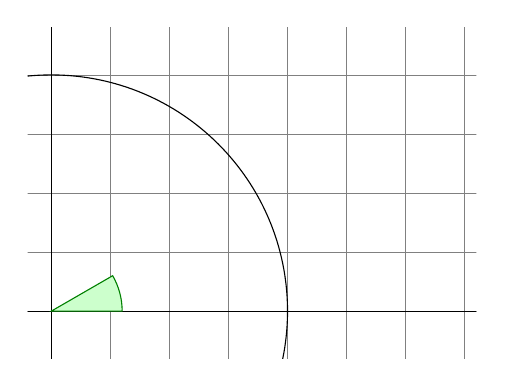
\begin{tikzpicture}[scale=3]
  \clip (-0.1,-0.2)
     rectangle (1.8,1.2);
  \draw[step=.25cm,gray,very thin]
       (-1.4,-1.4) grid (3.4,3.4);
  \draw (-1.5,0) -- (2.5,0);
  \draw (0,-1.5) -- (0,1.5);
  \draw (0,0) circle (1cm);
  \filldraw[fill=green!20!white,
            draw=green!50!black]
    (0,0) -- (3mm,0mm)
         arc (0:30:3mm) -- cycle;
\end{tikzpicture}
\end{example}
\noindent Tähele tuleks panna semikoolonit \texttt{;} käskude
eraldajana.

Lihtne Venni diagramm:
\begin{example}
\shorthandoff{:}
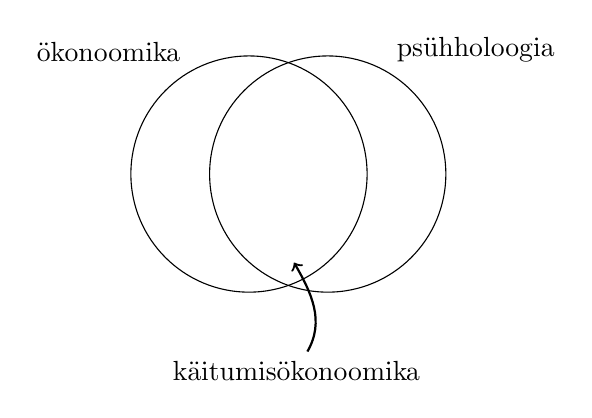
\begin{tikzpicture}
\node[circle,minimum size=3cm,
  draw,label=120:{ökonoomika}]
  at (0,0) {};
\node[circle,minimum size=3cm,
  draw,label=60:{psühholoogia}]
  at (1,0) {};
\node (i) at (0.5,-1) {};
\node at (0.6,-2.5)
  {käitumisökonoomika}
  edge[->,thick,out=60,in=-60](i);
\end{tikzpicture}
\end{example}
Kui paketti \pai{tikz} kasutatakse koos paketiga \pai{babel}, siis võib
juhtuda, et \pai{babel} muudab ümber mõne TikZi keele sümboli tähenduse,
mis toob kaasa kummalised vead. Selle vastu aitab tihti käsu
\ci{shorthandoff} lisamine koodi.

Järgmise näite iseärasus on tsükkel:

\begin{example}
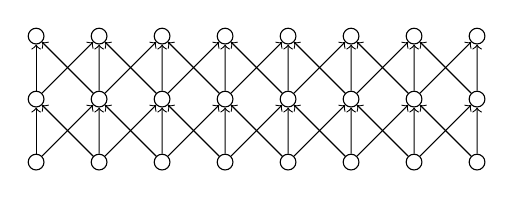
\begin{tikzpicture}[scale=0.8]
  \tikzstyle{v}=[circle,minimum size=2mm,inner sep=0pt,draw]
\foreach \i in {1,...,8}
\foreach \j in {1,...,3}
  \node[v](G-\i-\j) at (\i,\j){};
\foreach \i in {1,...,8}
\foreach \j/\o in {1/2,2/3}
  \draw[->](G-\i-\j)--(G-\i-\o);
\foreach \i/\n in
  {1/2,2/3,3/4,4/5,5/6,6/7,7/8}
  \foreach \j/\o in {1/2,2/3} {
    \draw[->] (G-\i-\j) -- (G-\n-\o);
    \draw[->] (G-\n-\j) -- (G-\i-\o); }
\end{tikzpicture}
\end{example}


Preambulis antava käsuga \ci{usetikzlibrary} saab aktiveerida laia skaala
lisavõimalusi erikujundite joonistamiseks, nagu see kergelt kumer kast:
\begin{example}
\usetikzlibrary{%
  decorations.pathmorphing}
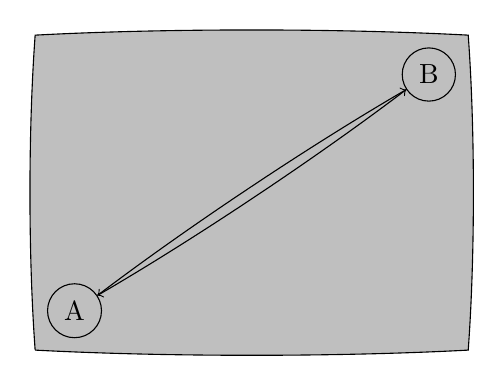
\begin{tikzpicture}[
     decoration={bent,aspect=.3}]
 \draw [decorate,fill=lightgray]
        (0,0) rectangle (5.5,4);
 \node[circle,draw]
        (A) at (.5,.5) {A};
 \node[circle,draw]
        (B) at (5,3.5) {B};
 \draw[->,decorate] (A) -- (B);
 \draw[->,decorate] (B) -- (A);
\end{tikzpicture}
\end{example}

\begin{example}
\usetikzlibrary{positioning}
\begin{tikzpicture}[xscale=6,
     yscale=8,>=stealth]
  \tikzstyle{v}=[circle,
     minimum size=1mm,draw,thick]
  \node[v] (a) {$1$};
  \node[v] (b) [right=of a] {$2$};
  \node[v] (c) [below=of a] {$2$};
  \node[v] (d) [below=of b] {$1$};
  \draw[thick,->]
        (a) to node {} (c);
  \draw[thick,->]
        (a) to node {} (d);
  \draw[thick,->]
        (b) to node {} (d);
\end{tikzpicture}
\end{example}

On isegi võimalik joonistada süntaksidiagramme, mis näevad välja nii,
nagu oleksid nad pärit otse Pascali programmeerimise õpikust. Kood on
eelmise näitega võrreldes veidi komplitseeritum, seetõttu on siin
esitatud ainult tulemus. Sellesama diagrammi joonistamiseks on paketi
\pai{pgf} dokumentatsioonis olemas üksikasjalik juhend.
\begin{center}
\begin{tikzpicture}[point/.style={coordinate},thick,draw=black!50,>=stealth',
                    tip/.style={->,shorten >=1pt},every join/.style={rounded corners},
                    skip loop/.style={to path={-- ++(0,#1) -| (\tikztotarget)}},
                    hv path/.style={to path={-| (\tikztotarget)}},
                    vh path/.style={to path={|- (\tikztotarget)}},
                 terminal/.style={
            rounded rectangle,
            minimum size=6mm,
            thick,draw=black!50,
            top color=white,bottom color=black!20,
            font=\ttfamily\tiny},
                nonterminal/.style={
                       rectangle,
                       minimum size=6mm,
                       thick,
                       draw=red!50!black!50,         % 50% red and 50% black,
                       top color=white,              % a shading that is white at the top...
                       bottom color=red!50!black!20, % and something else at the bottom
                       font=\itshape\tiny}]
\matrix[column sep=3.7mm] {
  % First row:
  & & & & & & & & & & & \node (plus) [terminal] {+};\\
  % Second row:
  \node (p1) [point] {}; &     \node (ui1)    [nonterminal] {märgita täisarv}; &
  \node (p2) [point] {}; &     \node (dot)    [terminal]    {.};                &
  \node (p3) [point] {}; &     \node (digit)  [terminal]    {number};            &
  \node (p4) [point] {}; &     \node (p5)     [point] {};                       &
  \node (p6) [point] {}; &     \node (e)      [terminal]    {E};                &
  \node (p7) [point] {}; &                                                      &
  \node (p8) [point] {}; &     \node (ui2)    [nonterminal] {märgita täisarv}; &
  \node (p9) [point] {}; &     \node (p10)    [point]       {};\\
  % Third row:
  & & & & & & & & & & & \node (minus)[terminal] {-};\\
};
{ [start chain]
  \chainin (p1);
  \chainin (ui1)   [join=by tip];
  \chainin (p2)    [join];
  \chainin (dot)   [join=by tip];
  \chainin (p3)    [join];
  \chainin (digit) [join=by tip];
  \chainin (p4)    [join];
  { [start branch=digit loop]
    \chainin (p3) [join=by {skip loop=-6mm,tip}];
  }
  \chainin (p5)    [join,join=with p2 by {skip loop=6mm,tip}];
  \chainin (p6)    [join];
  \chainin (e)     [join=by tip];
  \chainin (p7)    [join];
  { [start branch=plus]
    \chainin (plus) [join=by {vh path,tip}];
    \chainin (p8)    [join=by {hv path,tip}];
  }
  { [start branch=minus]
    \chainin (minus) [join=by {vh path,tip}];
    \chainin (p8)    [join=by {hv path,tip}];
  }
  \chainin (p8)    [join];
  \chainin (ui2)   [join=by tip];
  \chainin (p9)    [join,join=with p6 by {skip loop=-11mm,tip}];
  \chainin (p10)   [join=by tip];
}
\end{tikzpicture}
\end{center}

Võimalusi on veelgi: kui tuleb joonistada arvuliste andmete või
funktsioonide graafikuid, siis võib vaadata paketti \pai{pgfplot}, mis
sisaldab kõike, mida graafikute joonistamisel vaja läheb. See pakett
suudab isegi kutsuda välja välise \wi{Gnuplot}i käsu, et välja arvutada
graafikusse kirjutatud funktsiooni tegelik väärtus.

Veel rohkem inspiratsiooni annab \index{Fauske, Kjell Magne}Kjell Magne
Fauske suurepärane \url{http://www.texample.net/tikz}, kust leiab
pidevalt täieneva kogu ilusaid jooniseid ja muud \LaTeX i koodi. Samal
\index{texample.net@\TeX{}ample.net}\TeX{}ample.net-i lehel on väljas ka
mitmesuguste PGFi/TikZi tööriistade nimekiri
(\url{http://www.texample.net/tikz/resources/#tools-that-generate-pgftikz-code}),
nii et ei ole vaja kirjutada kogu koodi käsitsi.

%%% Local Variables:
%%% TeX-master: "lshort.tex"
%%% mode: flyspell
%%% TeX-PDF-mode: t
%%% End:
